\documentclass[10pt]{article}

% Default 
\usepackage{graphicx}
\usepackage[
  backend=biber,
  style=numeric, 
  sorting=none
]{biblatex}

% Additional
\usepackage{amsmath}
\usepackage{textcomp}
\usepackage{gensymb}
\usepackage{placeins}
\usepackage{tabularray} 
\usepackage{xcolor}
\usepackage{placeins}
\usepackage{csquotes} 
\usepackage{todonotes}
\usepackage{hyperref}
\usepackage{siunitx}

\newcommand{\td}[1]{\todo[linecolor=blue, backgroundcolor=blue!25,bordercolor=blue, size=\small, inline]{#1}}

\addbibresource{references.bib}

\title{Reflection} 
\author{Rahmanyaz Annyyev, Hikmat Gulaliyev}
\date{16 May, 2024} 

\begin{document}

\maketitle

\begin{abstract}
In this experiment, the validity of Fresnel's equations is tested by measuring the intensity of reflected light at different angles of incidence for both s- and p-polarizations, computing the ratio of both parallel and perpendicular components of light, and comparing the results with the theoretical values via plotting the data. The Brewster angle is calculated by first measuring the transmission angle at different angles of incidence, plotting the data, and finding the refractive index of the cylindrical block. 
\end{abstract}

\section{Introduction}

\subsection*{General}

When electromagnetic radiation strikes an interface between two different optical media, a fraction of the radiation is reflected and the rest is transmitted. Fresnel's equations, or coefficients of reflection and transmission, quantitatively describe the behavior of light at the interface between two media. 

The amplitude reflection coefficient, denoted by $r$, is the ratio of the reflected wave's amplitude to the incident wave's amplitude. The amplitude transmission coefficient, denoted by $t$, is the ratio of the transmitted wave's amplitude to the incident wave's amplitude. They are given by the following equations:
\begin{equation}
  r = \frac{E_{0r}}{E_{0i}} \quad \text{and} \quad t = \frac{E_{0t}}{E_{0i}}
\end{equation}
where $E_{0r}$, $E_{0i}$, and $E_{0t}$ are the amplitudes of the reflected, incident, and transmitted waves, respectively.

These coefficients are derived from the boundary conditions of the electric and magnetic fields at the interface between the two media. The values of the coefficients depend on the angle of incidence, the refractive indices of the two media, and most importantly, the polarization of the incident light. Let the refractive indices of the incident and transmitted media be $n_i$ and $n_t$, respectively, and let the angle of incidence, reflectance, and transmittance be $\theta_i$, $\theta_r$, and $\theta_t$, respectively \cite{Pedrotti_2006}.

There are two types of polarization: s-polarization and p-polarization. In s-polarization, the electric field vector is perpendicular to the plane of incidence, and the coefficients are given by the following equations:
\begin{equation}
  r_{\perp} \equiv \left(\frac{E_{0r}}{E_{0i}}\right)_{\perp} = \frac{n_i \cos(\theta_i) - n_t \cos(\theta_t)}{n_i \cos(\theta_i) + n_t \cos(\theta_t)}
\end{equation}
and
\begin{equation}
  t_{\perp} \equiv \left(\frac{E_{0t}}{E_{0i}}\right)_{\perp} = \frac{2n_i \cos(\theta_i)}{n_i \cos(\theta_i) + n_t \cos(\theta_t)}
\end{equation}
where the subscripts $\perp$ denote s-polarization. In p-polarization, the electric field vector is parallel to the plane of incidence, and the coefficients are given by the following equations:
\begin{equation}
  r_{\parallel} \equiv \left(\frac{E_{0r}}{E_{0i}}\right)_{\parallel} = \frac{n_t \cos(\theta_i) - n_i \cos(\theta_t)}{n_t \cos(\theta_i) + n_i \cos(\theta_t)}
\end{equation}
and
\begin{equation}
  t_{\parallel} \equiv \left(\frac{E_{0t}}{E_{0i}}\right)_{\parallel} = \frac{2n_i \cos(\theta_i)}{n_t \cos(\theta_i) + n_i \cos(\theta_t)}
\end{equation}
where the subscripts $\parallel$ denote p-polarization \cite{Hecht_2017}.

The angles of incidence and transmission are related by Snell's law, which states that the refractive indices of the two media and the sines of the angles of incidence and transmission are related by the following equation:
\begin{equation}
  n_i \sin(\theta_i) = n_t \sin(\theta_t)
\end{equation}
By performing a series of algebraic manipulations, the reflection coefficients can be brought into the following forms:
\begin{equation}
  r_{\perp} = -\frac{\sin(\theta_i - \theta_t)}{\sin(\theta_i + \theta_t)}
\end{equation}
and 
\begin{equation}
  r_{\parallel} = \frac{\tan(\theta_i - \theta_t)}{\tan(\theta_i + \theta_t)}
\end{equation}

At a certain angle of incidence, known as the Brewster angle, the reflection coefficient for p-polarization becomes zero. This angle is given by the following equation:
\begin{equation}
  \theta_B = {\arctan}{\left(\frac{n_t}{n_i}\right)}
\end{equation}

\subsection*{Procedure} 

The setup consists of an optical bench, two polarizers, an angular translator, a light-sensitive detector, a laser, a slit collimator, an interface, and a square analyzer.

The purpose of the experiment is to find refraction angles and intensities of parallel and perpendicular components of light at different incident angles.

Before starting the experiment setup needs to be calibrated. To do so we first need to mount the slit collimator away from the laser. After putting the slit collimator to configuration $\#5$, we set the angle of the angle translator to $0\degree$. Now, we can align the laser using its alignment screws to make sure the laser beam passes through the center of the detector aperture. 

After mounting polarizers on and setting the angle of polarizer $\#2$ to $45\degree$ to divide light into two linear electric field components that are perpendicular to each other, we can turn the interface on. Selecting the Light Sensor, and opening the METER icon, enables us to measure light intensity. However, the interface needs to be calibrated as well, by resetting the meter, and later adjusting the intensity of polarizer $\#1$ so that the maximum reading is not more than $100\%$.

We can now put the cylindrical lens on the pivot plate and align it with the angular translator and pivot plane so that the flat surface faces the laser beam. Rotating the plates will now result in reflection and refraction at the dielectric interface that is formed between air and the flat surface.

Now we can set the incident angle at different values by turning the angular translator, and find the refraction angle by again rotating the angular translator so that intensity is maximum. After noting the angle in Table 1. We can put in the square analyzer to also record horizontal and vertical components of light. Also by finding points where horizontal intensity is zero, we can find Brewster's angle.
 
\section{Data \& Results}

From the slope of the best-fit line in Figure~(\ref{fig:f1}), the refractive index of the cylindrical block is calculated to be $1.30$. The Brewster angle is calculated to be $52.4\degree$.

\begin{table}[ht]
  \centering
  \begin{tblr}{
    cells = {halign = c, valign = m},
    column{1-2} = {bg = lightgray!20},
    hlines = {},
    vlines = {}
  }
    $\theta_i$ & $20\degree$ & $30\degree$ & $40\degree$ & $50\degree$ & $60\degree$ & $70\degree$ & $80\degree$ \\
    $\theta_t$ & $7\degree$ & $10\degree$ & $14\degree$ & $18\degree$ & $23\degree$ & $30\degree$ & $37\degree$ 
  \end{tblr}
  \caption{Incident and transmission angles.}
  \label{tab:1}
\end{table}

\begin{figure}[h]
  \centering
  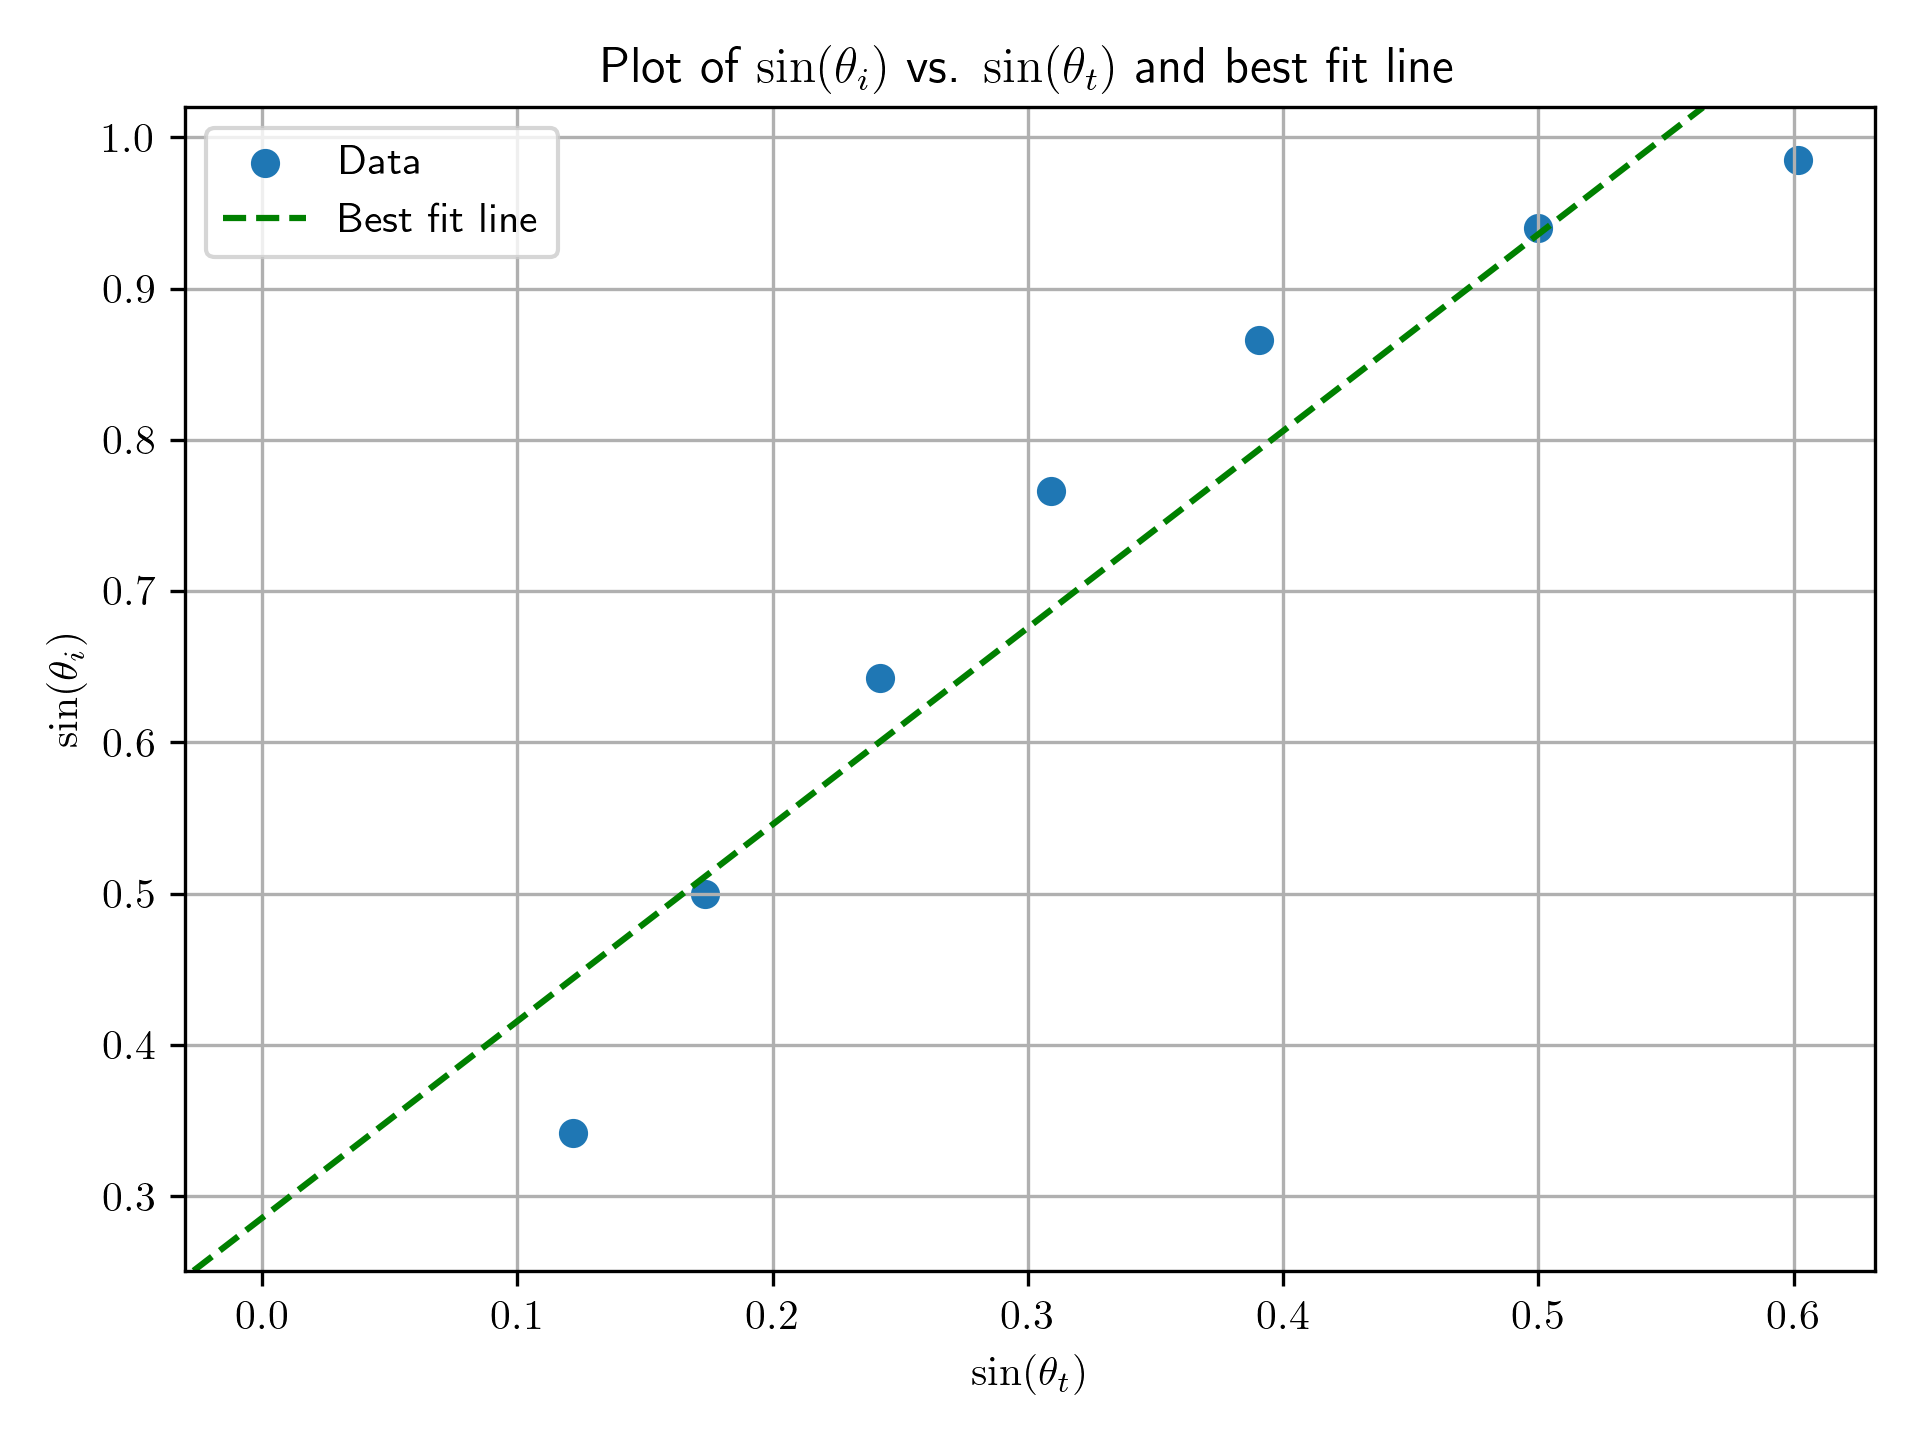
\includegraphics[scale=0.7]{plots/p1.png}
  \caption{Plot of $\sin(\theta_i)$ vs. $\sin(\theta_t)$ and best fit line.}
  \label{fig:f1}
\end{figure}

\begin{table}[ht]
  \centering
  \tiny
  \begin{tblr}{
    cells = {halign = c, valign = m},
    column{1-2} = {bg = lightgray!20},
    hlines = {},
    vlines = {}
  }
    $\theta_i$ & $20\degree$ & $25\degree$ & $30\degree$ & $35\degree$ & $40\degree$ & $45\degree$ & $50\degree$ & $55\degree$ & $60\degree$ & $65\degree$ & $70\degree$ & $75\degree$ & $80\degree$ \\
    $I(\theta_i)_\parallel$ & $33$ & $22$ & $25$ & $25$ & $19$ & $17$ & $9$ & $6$ & $3$ & $6$ & $5$ & $4$ & $3$ \\
  \end{tblr}
  \caption{Reflection intensities for p-polarization.}
  \label{tab:2}
\end{table}

\begin{table}[ht]
  \centering
  \tiny
  \begin{tblr}{
    cells = {halign = c, valign = m},
    column{1-2} = {bg = lightgray!20},
    hlines = {},
    vlines = {}
  }
    $\theta_i$ & $20\degree$ & $25\degree$ & $30\degree$ & $35\degree$ & $40\degree$ & $45\degree$ & $50\degree$ & $55\degree$ & $60\degree$ & $65\degree$ & $70\degree$ & $75\degree$ & $80\degree$ \\
    $I(\theta_i)_\perp$ & $33$ & $22$ & $25$ & $25$ & $19$ & $17$ & $9$ & $6$ & $3$ & $6$ & $5$ & $4$ & $3$ \\
  \end{tblr}
  \caption{Reflection intensities for s-polarization.}
  \label{tab:3}
\end{table}

\begin{figure}[h]
  \centering
  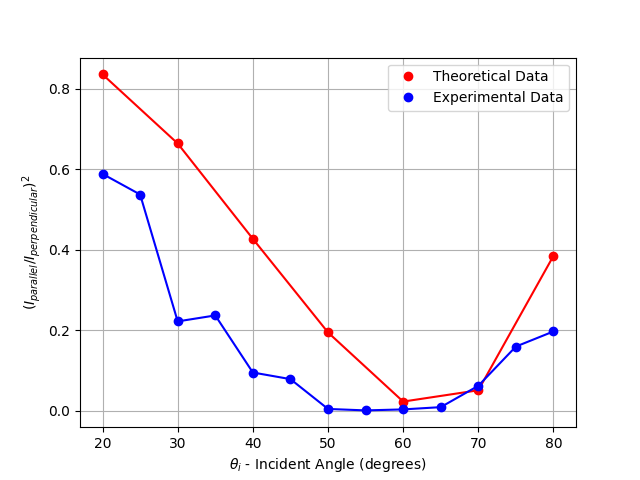
\includegraphics[scale=0.7]{plots/p2.png}
  \caption{Plot of $\left(r_{\parallel}/r_{\perp}\right)^2$ and $I_{\parallel}/I_{\perp}$ vs. $\theta_i$.}
  \label{fig:f2}
\end{figure}

\section{Discussion \& Conclusion}

\subsection*{Errors}
The sources of error for this experiment are calibration error, human error, and imperfect instrumentation.
\begin{itemize}
  \item \textbf{Calibration error:} Calibration of the light sensor was unsuccessful at times, as the intensity was exceeding $100\%$, causing the readings to go out of the detection range. Additionally, the calibration of the laser into the aperture was done by hand, and it did not always fall directly into the aperture, which affected intensity measurements.
  \item \textbf{Human error:} All measurements, alignments, and angle determinations were done by hand, and therefore may not be accurate.
  \item \textbf{Imperfect instrumentation:} The biggest source of error was imperfect instrumentation. The plates were moving relative to each other while using the angular translator, which changed the incident and reflection angles, thereby affecting intensities immensely.
\end{itemize}

\subsection*{Approximations}
\begin{itemize}
  \item \textbf{Refractive index of the air:} The refractive index of the air was assumed to be $1$.
  \item \textbf{Homogenity of the block:} The block was assumed to be homogenous.
  \item \textbf{Coherence of the light:} The light was assumed to be coherent.
  \item \textbf{Homogenity of the medium:} Medium in which the laser was traveling was assumed to be homogenous.
\end{itemize}

\subsection*{Discrepancies}

\subsection*{Conclusion} 

\section{Extra Credit}

Fresnel equations are a powerful tool for understanding the behavior of light at the interface of two media. They are used in many applications, such as the design of anti-reflective coatings, the study of thin films, and the design of optical components. One of the most common applications of Fresnel equations is in the design of LCDs. By controlling the polarization of light, we can control the intensity of light that passes through the display, allowing us to create images with high contrast and brightness \cite{dePooter_2002}.

\printbibliography

\end{document}